Dans un réacteur nucléaire se trouve le coeur constitué de crayons de combustible (principalement de plutonium et d'uranium). Ces crayons sont assemblés à l'aide de gaines et sont placés dans le réacteur. Un circuit complexe d'eau est ensuite installé et permet de faire passer l'eau à l'intérieur de ces gaines. La réaction de fission de l'uranium et du plutonium va provoquer l'émission de particules hautement énergétiques qui vont chauffer l'eau dans le circuit. L'eau va ensuite passer dans un pressuriseur et se transformera en vapeur qui fera tourner plusieurs turbines, ce qui va provoquer la production d'électricité (voir figure~\ref{reacteur}). Le fonctionnement d'un 
réacteur nucléaire est bien sur bien plus complexe que cela, mais dans le cadre du stage, le fonctionnement en détail du réacteur n'a pas besoin d'être connu, le principal étant de comprendre qu'à l'intérieur du coeur du réacteur se trouve des crayons de combustible, et que ce sont ces crayons qui vont pouvoir provoquer les accidents graves.\\

\begin{figure}[h]
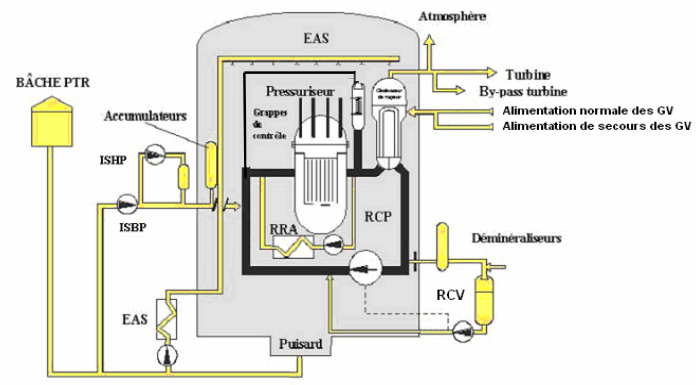
\includegraphics[scale=0.5]{reacteur.png}
\caption{Schéma d'un réacteur nucléaire}
\label{reacteur}
\end{figure}


Un crayon est formé de combustible (uranium et plutonium), mais aussi d'une gaine en Zirconium pour maintenir les pastilles de combustible ensemble. Un accident grave est généralement causé par un problème de refroidissement de ces crayons de combustible dont la puissance résiduelle ne pourra plus être efficacement évacuée. Ces crayons vont alors fondre et former un mélange appelé corium principalement formé de zirconium, d'uranium,de plutonium et parfois de nickel et de chrome venant des installations. La température peut dépasser les 2800K. L'étude de ce mélange est centrale dans l'approche des accidents graves : du fait de sa forte teneur en élément radioactif, ce mélange est destructeur et la propagation de ce mélange peut être fatale à toute l'installation. Le corium se propage alors dans la cuve, puis s'il détruit la cuve, se propage dans le bâtiment du réacteur, et, encore plus grave,à l'éxtérieur du réacteur s'il détruit la structure généralement en béton de celui-ci. Ainsi, en se propageant, le corium réagit avec les différents éléments du réacteur et plusieurs types d'intéraction peuvent alors se produire : intéraction avec l'eau froide du réacteur (ICE), ou encore intéraction avec le béton du fond du réacteur (ICB).  Lorsque le corium commence à se propager dans le réacteur, il y a ainsi de forte chance pour que le réacteur ne puisse plus jamais fonctionner, le but n'est donc pas d'essayer de sauvegarder le réacteur mais de prévenir toute perte humaine. \\

Dans le domaine des accidents graves, les phénomènes physiques mis en jeu sont trés complexes et ne peuvent être bien étudiés à l'heure actuelle. La but de l'étude des accidents graves est de comprendre au mieux ces 
phénomènes, de produire des codes de simulation qui pourront prévoir, toujours au mieux, le comportement du corium mais aussi et sutout d'essayer de majorer l'erreur comise lors de telles simulations. Comme dit précédemment,
les données concernant les accidents graves sont actuellement trés limitées et il est trés difficile de produite de nouvelles données. On peut récupérer des données de prédents accidents (Three Mile Island, Fukushima, Tchernobyl),
ou encore faire des simulations à échelle réduite (installation PLINIUS au Cea Cadarache par exemple). Les codes scénario permettent ainsi de simuler la propagation du corium au sein de l'enceinte du réacteur. Le code PROCOR 
est le code développé au laboratoire LPMA du Cea Cadarache où se déroule le stage. C'est un code orienté objet en Java permettant de créer des applications PROCOR prenant différents modèles (comme un modèle de cuve, un modèle 
de corium) et permettant de simuler les intéractions entre ces modèles. Ainsi une application PROCOR prend la forme d'un système dynamique qui évolue au cours du temps, ce système dynamique étant composé de plusieurs modèles
et d'un ensemble d'intéraction entre ces modèles. Chaque modèle peut évoluer pendant le cycle de vie de l'application, il peut être détruit si par exemple un élément comme le corium détruit une enceinte. La plateforme permet,
 par le biais de méthodes de Monte-Carlo d'obtenir des probabilités de rupture de cuve, ou plus généralement permet d'avoir des résultats de sensibilité sur certain paramètre physique et d'incertitude sur certains matériaux. 